After a model is trained, the first following step is model selection then
assessment.  Selection is estimating model performance among a set of trained
models using a single validation set.  After one model is chosen, assessment
takes place by determining the prediction capability on new data via a
previously unseen testing set. Both selection and assessment can be done in a
single step using \textit{k}-fold cross-validation, which is described below.

\subsubsection{Sources of Error} 

The bias is error from erroneous
assumptions in the learning algorithm. High bias can cause an algorithm to miss
the relevant relations between features and target outputs (underfitting).  

The
variance is error from sensitivity to small fluctuations in the training set.
High variance can cause an algorithm to model the random noise in the training
data, rather than the intended outputs (overfitting).

\begin{figure}[!htb]
  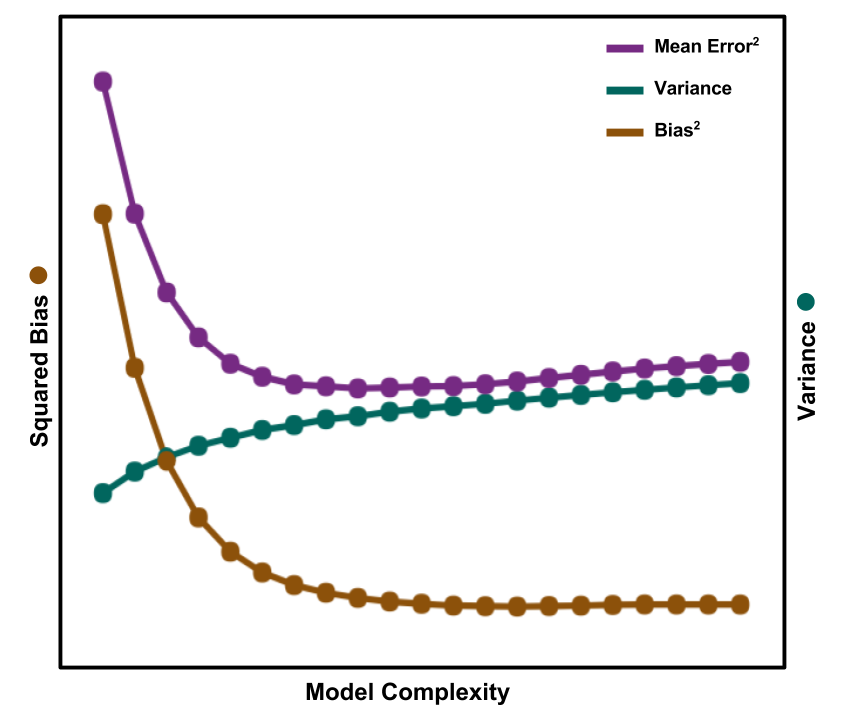
\includegraphics[width=\linewidth]{./chapters/litrev/BVtradeoff.png}
  \caption{Model prediction error shown to be comprised of bias and variance}
  \label{fig:bvtradeoff}
\end{figure}

\subsubsection{Types of Error}

%%%%%%%%%%%%%%%%%%%%%%%%%%%%%%%%%%%%%%%%%%%%%%%%%%%%%%%%%%%%
%%%%%%%%%%%%%%%%%%%%%%%%%%%%%%%%%%%%%%%%%%%%%%%%%%%%%%%%%%%%
Discuss J functions (target function, objective function) and
how that is essentially error the alg is trying to minimize. 
%%%%%%%%%%%%%%%%%%%%%%%%%%%%%%%%%%%%%%%%%%%%%%%%%%%%%%%%%%%%
%%%%%%%%%%%%%%%%%%%%%%%%%%%%%%%%%%%%%%%%%%%%%%%%%%%%%%%%%%%%

Evaluating the generalization (i.e., prediction capability) of a
machine-learned model is important because the creation of statistically
learned models is a hidden process. This is done by taking a small portion of
the data set, and setting it aside as a testing set.  The rest of the data set
is known as the training set and is used to train a model. After training, the
test set is used to test the model.  

The generalization error is typically referred to as the \textit{testing
error}, as it is measuring the ability of the model to predict future cases
that were not introduced in the training phase (i.e., the testing set entries).
Next, the \textit{training error} is provided by comparing the model
predictions to the training set, as the model would likely be smoother than the
potential noise the training set would include. This is useful to determine the
fitness of the model, the application of which is discussed below in Section
\ref{sec:optvalid}.

Although one could just train and test their model, there is a way to test the
model while still in the training phase. A testing set that would be used
during training to give feedback, a \textit{cross-validation} set, can provide
a faster convergence to a satisfactory model. As shown in Figure
\ref{fig:cverror}, this can be done by splitting the data set into three
groups: a large training set, a small cross-validation set, and a small testing
set. 

\begin{figure}[!htb]
  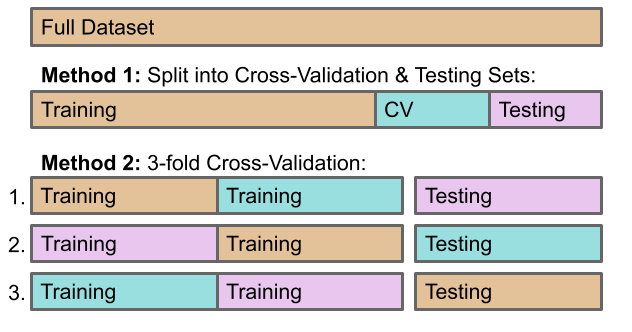
\includegraphics[width=\linewidth]{./chapters/litrev/cverror.png}
  \caption{Illustration of how a dataset can be split up for model evaluation}
  \label{fig:cverror}
\end{figure}

However, in practice, multiple rounds of cross-validation steps are used,
referred to as \textit{k-fold cross-validation}. This allows a user to use all
data entries as a testing entry once.  As illustrated in \ref{fig:cverror},
this splits the dataset into \textit{k} subsets. One set is designated as the
testing set, and a model is trained with the rest. Following the first training
phase, another begins, this time with a different subset as the testing set.
This process is performed \textit{k} times to give \textit{k} models, and the
models are then averaged, providing an additional level of model validation
than can be achieved with a single testing set.

